\documentclass[11pt,a4paper]{article}

\usepackage[utf8]{inputenc}
\usepackage[T1]{fontenc}
\usepackage{amsmath,amssymb,amsthm}
\usepackage{listings}
\usepackage{xcolor}
\usepackage{tikz}
\usetikzlibrary{shapes,arrows,positioning,fit,calc}
\usepackage{hyperref}
\usepackage{algorithm}
\usepackage{algpseudocode}
\usepackage{booktabs}
\usepackage{geometry}
\usepackage{fancyhdr}
\usepackage{tocloft}

\geometry{margin=1in}

% Code listing styles
\definecolor{codegreen}{rgb}{0,0.6,0}
\definecolor{codegray}{rgb}{0.5,0.5,0.5}
\definecolor{codepurple}{rgb}{0.58,0,0.82}
\definecolor{backcolour}{rgb}{0.95,0.95,0.92}

\lstdefinestyle{zkasm}{
    backgroundcolor=\color{backcolour},
    commentstyle=\color{codegreen},
    keywordstyle=\color{blue}\bfseries,
    numberstyle=\tiny\color{codegray},
    stringstyle=\color{codepurple},
    basicstyle=\ttfamily\small,
    breakatwhitespace=false,
    breaklines=true,
    captionpos=b,
    keepspaces=true,
    numbers=left,
    numbersep=5pt,
    showspaces=false,
    showstringspaces=false,
    showtabs=false,
    tabsize=2,
    morekeywords={fn,pub,const,var,if,goto,return,include},
    morecomment=[l]{;;}
}

\lstdefinestyle{golang}{
    backgroundcolor=\color{backcolour},
    commentstyle=\color{codegreen},
    keywordstyle=\color{blue}\bfseries,
    numberstyle=\tiny\color{codegray},
    stringstyle=\color{codepurple},
    basicstyle=\ttfamily\small,
    breakatwhitespace=false,
    breaklines=true,
    captionpos=b,
    keepspaces=true,
    numbers=left,
    numbersep=5pt,
    showspaces=false,
    showstringspaces=false,
    showtabs=false,
    tabsize=2,
    morekeywords={func,type,struct,interface,return,if,else,for,range,package,import,var,const,map,make,append,len,uint,int,string,bool,error,nil}
}

\pagestyle{fancy}
\fancyhf{}
\rhead{zkASM Technical Report}
\lhead{go-corset}
\rfoot{Page \thepage}

\title{\textbf{zkASM: A Zero-Knowledge Assembly Language}\\[0.5em]
\large Technical Report on the go-corset Implementation}
\author{Generated from go-corset source analysis}
\date{\today}

\begin{document}

\maketitle

\begin{abstract}
This technical report provides a comprehensive analysis of zkASM, a zero-knowledge assembly language implemented within the go-corset compiler framework. zkASM serves as an intermediate representation that bridges high-level constraint specifications with low-level arithmetic circuits suitable for zero-knowledge proof systems. We examine the language syntax, compilation pipeline, constraint generation mechanisms, and field-agnostic execution model. The report details the novel register splitting algorithm for field independence, the vectorization optimization pass, and the bus-based inter-function communication protocol.
\end{abstract}

\tableofcontents
\newpage

%==============================================================================
\section{Introduction}
%==============================================================================

\subsection{Background and Motivation}

Zero-knowledge proof systems require arithmetic constraints over finite fields to be expressed in a specific format amenable to cryptographic protocols. The go-corset project provides a compilation framework that transforms human-readable constraint specifications into optimized arithmetic intermediate representations (AIR).

zkASM (Zero-Knowledge Assembly) is a low-level programming language within this framework that provides:
\begin{itemize}
    \item Explicit control over register allocation and data flow
    \item Direct mapping to arithmetic constraints
    \item Field-agnostic programming with automatic adaptation
    \item Efficient function composition via I/O buses
\end{itemize}

\subsection{Document Organization}

This report is organized as follows:
\begin{itemize}
    \item Section 2 presents the zkASM language syntax and semantics
    \item Section 3 details the compilation pipeline architecture
    \item Section 4 explains the constraint generation process
    \item Section 5 describes the field-agnostic execution model
    \item Section 6 covers the executor and trace generation
    \item Section 7 discusses integration with the broader constraint system
    \item Section 8 provides implementation details and algorithms
\end{itemize}

%==============================================================================
\section{zkASM Language Specification}
%==============================================================================

\subsection{Lexical Structure}

The zkASM lexer recognizes the following token categories:

\begin{table}[h]
\centering
\begin{tabular}{lll}
\toprule
\textbf{Category} & \textbf{Tokens} & \textbf{Examples} \\
\midrule
Keywords & \texttt{fn}, \texttt{pub}, \texttt{const}, \texttt{var}, \texttt{if}, \texttt{goto}, \texttt{return} & \\
Types & \texttt{u1}, \texttt{u8}, \texttt{u16}, \texttt{u32}, \texttt{u128}, \texttt{u256} & \\
Operators & \texttt{+}, \texttt{-}, \texttt{*}, \texttt{/}, \texttt{==}, \texttt{!=}, \texttt{<}, \texttt{>} & \\
Delimiters & \texttt{(}, \texttt{)}, \texttt{\{}, \texttt{\}}, \texttt{,}, \texttt{:} & \\
Literals & Numbers (decimal, hex, binary) & \texttt{42}, \texttt{0xFF}, \texttt{0b1010} \\
Comments & Line comments & \texttt{;; comment} \\
\bottomrule
\end{tabular}
\caption{zkASM Token Categories}
\end{table}

\subsection{Type System}

zkASM uses unsigned integer types with explicit bit widths:

\begin{equation}
\text{Type} ::= \texttt{u}n \quad \text{where } n \in \{1, 8, 16, 32, 64, 128, 256\}
\end{equation}

Each type $\texttt{u}n$ represents values in the range $[0, 2^n - 1]$. The type system enforces:
\begin{itemize}
    \item Arithmetic operations preserve or extend bit widths
    \item Carry/overflow bits are explicitly captured
    \item Division produces quotient, remainder, and witness values
\end{itemize}

\subsection{Function Declarations}

Functions are declared with explicit input/output signatures:

\begin{lstlisting}[style=zkasm,caption={Function Declaration Syntax}]
fn function_name(param1 type1, param2=default type2)
    -> (out1 type3, out2=padding type4) {
    ;; function body
    return
}
\end{lstlisting}

Key features:
\begin{itemize}
    \item \textbf{Default values}: Parameters can specify default values for padding
    \item \textbf{Multiple outputs}: Functions return multiple values with explicit types
    \item \textbf{Padding values}: Output padding values are used for trace expansion
\end{itemize}

\subsection{Register Declarations}

Internal registers are declared with the \texttt{var} keyword:

\begin{lstlisting}[style=zkasm,caption={Register Declarations}]
var counter u32          ;; Single register
var flag1, flag2 u1      ;; Multiple registers of same type
var temp u16             ;; Temporary computation register
\end{lstlisting}

\subsection{Instruction Set}

\subsubsection{Assignment Instructions}

Assignments compute expressions and store results:

\begin{lstlisting}[style=zkasm,caption={Assignment Examples}]
result = input1 + input2           ;; Simple addition
carry, sum = a + b                 ;; Addition with carry capture
q, r, w, s, ws = dividend / divisor ;; Division with full outputs
\end{lstlisting}

The assignment semantics for addition with carry:
\begin{equation}
\texttt{carry} \cdot 2^n + \texttt{sum} = a + b
\end{equation}
where $n$ is the bit width of \texttt{sum}.

\subsubsection{Control Flow Instructions}

\begin{lstlisting}[style=zkasm,caption={Control Flow Examples}]
;; Conditional branch
if counter == 0 goto exit_label

;; Unconditional branch
goto loop_start

;; Labels
loop_start:
    ;; instructions
exit_label:
    return
\end{lstlisting}

Supported comparison operators: \texttt{==}, \texttt{!=}, \texttt{<}, \texttt{<=}, \texttt{>}, \texttt{>=}

\subsubsection{Function Calls}

Inter-function communication uses I/O buses:

\begin{lstlisting}[style=zkasm,caption={Function Call Example}]
;; Call another function
result = other_function(arg1, arg2)

;; Multiple return values
quot, rem = divide(dividend, divisor)
\end{lstlisting}

\subsubsection{Ternary Expressions}

Conditional expressions for compact logic:

\begin{lstlisting}[style=zkasm,caption={Ternary Expression}]
result = condition == 1 ? true_value : false_value
\end{lstlisting}

\subsection{Complete Example}

\begin{lstlisting}[style=zkasm,caption={Division Function Implementation}]
fn div(x u16, y=1 u16) -> (q u16, r u16) {
    var sum u32
    var wit u16
    var witsum u17

    ;; Compute division with witness
    q, r, wit, sum, witsum = x / y
    return
}
\end{lstlisting}

The division operation generates constraints:
\begin{align}
\texttt{sum} &= q \cdot y + r \\
\texttt{witsum} &= r + \texttt{wit} + 1 \\
\texttt{sum} &= x \\
\texttt{witsum} &= y
\end{align}

These constraints ensure $q = \lfloor x/y \rfloor$ and $r = x \mod y$ with $r < y$.

%==============================================================================
\section{Compilation Pipeline}
%==============================================================================

\subsection{Pipeline Overview}

The zkASM compilation pipeline transforms source code through multiple intermediate representations:

\begin{figure}[h]
\centering
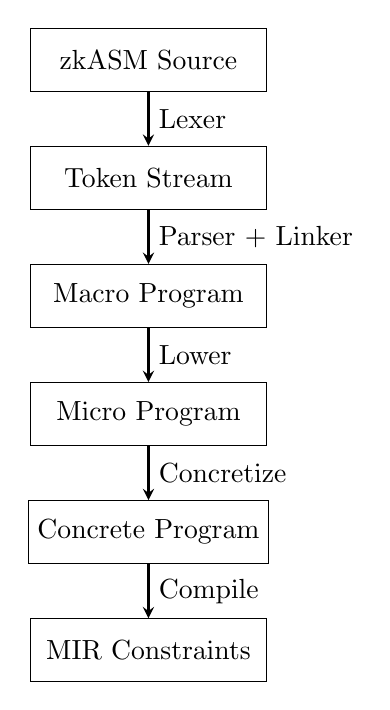
\begin{tikzpicture}[
    node distance=1.5cm,
    box/.style={rectangle, draw, minimum width=3cm, minimum height=0.8cm, align=center},
    arrow/.style={->, >=stealth, thick}
]
    \node[box] (source) {zkASM Source};
    \node[box, below of=source] (tokens) {Token Stream};
    \node[box, below of=tokens] (macro) {Macro Program};
    \node[box, below of=macro] (micro) {Micro Program};
    \node[box, below of=micro] (concrete) {Concrete Program};
    \node[box, below of=concrete] (mir) {MIR Constraints};

    \draw[arrow] (source) -- node[right] {Lexer} (tokens);
    \draw[arrow] (tokens) -- node[right] {Parser + Linker} (macro);
    \draw[arrow] (macro) -- node[right] {Lower} (micro);
    \draw[arrow] (micro) -- node[right] {Concretize} (concrete);
    \draw[arrow] (concrete) -- node[right] {Compile} (mir);
\end{tikzpicture}
\caption{zkASM Compilation Pipeline}
\end{figure}

\subsection{Lexical Analysis}

The lexer (\texttt{assembler/lexer.go}) tokenizes source files into a stream of tokens. Key features:

\begin{itemize}
    \item Support for multiple number formats (decimal, hexadecimal \texttt{0x}, binary \texttt{0b})
    \item Underscore separators in numeric literals for readability
    \item Line comments with \texttt{;;}
    \item Source location tracking for error reporting
\end{itemize}

\subsection{Parsing and Linking}

The parser (\texttt{assembler/parser.go}) constructs an abstract syntax tree representing:

\begin{itemize}
    \item Function declarations with register specifications
    \item Instruction sequences with label resolution
    \item Expression trees for computations
\end{itemize}

The linker (\texttt{assembler/linker.go}) performs:

\begin{itemize}
    \item \textbf{Bus Resolution}: Maps function names to unique bus identifiers
    \item \textbf{Constant Substitution}: Replaces named constants with values
    \item \textbf{Cross-file References}: Resolves inter-file function calls
\end{itemize}

\subsection{Validation}

The validator (\texttt{assembler/validation.go}) performs two-phase checking:

\textbf{Phase 1 - Instruction Validation:}
\begin{itemize}
    \item Register bit-width balance verification
    \item Signed arithmetic carry bit validation
    \item Field width requirement checking
\end{itemize}

\textbf{Phase 2 - Control Flow Analysis:}
\begin{itemize}
    \item Reachability analysis (all paths reach \texttt{return})
    \item Uninitialized register detection
    \item Label definition verification
    \item Input register write prevention
\end{itemize}

\subsection{Macro to Micro Lowering}

The lowering phase transforms high-level macro instructions into primitive micro instructions:

\begin{table}[h]
\centering
\begin{tabular}{ll}
\toprule
\textbf{Macro Instruction} & \textbf{Micro Expansion} \\
\midrule
\texttt{Assign} & \texttt{Assign} + \texttt{Jmp} \\
\texttt{IfGoto} & \texttt{Skip} + \texttt{Jmp} + \texttt{Jmp} \\
\texttt{Division} & \texttt{Division} + \texttt{Assign}$\times 2$ + \texttt{Skip}$\times 2$ + \texttt{Jmp} + \texttt{Fail} \\
\texttt{Call} & \texttt{InOut} + \texttt{Jmp} \\
\texttt{Return} & \texttt{Ret} \\
\texttt{Goto} & \texttt{Jmp} \\
\bottomrule
\end{tabular}
\caption{Macro to Micro Instruction Mapping}
\end{table}

\subsection{Vectorization Optimization}

The vectorization pass merges consecutive non-conflicting instructions:

\begin{algorithm}
\caption{Instruction Vectorization}
\begin{algorithmic}[1]
\Function{Vectorize}{instructions}
    \For{each instruction $i$ at PC $p$}
        \State $conflicts \gets \emptyset$
        \State $merged \gets \{i\}$
        \For{each following instruction $j$ at PC $p+k$}
            \If{$\text{WritesConflict}(merged, j)$}
                \State \textbf{break}
            \EndIf
            \State $merged \gets merged \cup \{j\}$
        \EndFor
        \State $instructions[p] \gets \text{MergeInstructions}(merged)$
    \EndFor
    \State \Return \Call{PruneUnreachable}{instructions}
\EndFunction
\end{algorithmic}
\end{algorithm}

Conflict detection prevents merging when:
\begin{itemize}
    \item Multiple instructions write to the same register
    \item Branch targets land in the middle of a merged instruction
\end{itemize}

%==============================================================================
\section{Constraint Generation}
%==============================================================================

\subsection{Constraint Model}

Each micro instruction generates polynomial constraints over finite field $\mathbb{F}$:

\begin{definition}[Vanishing Constraint]
A vanishing constraint is a polynomial $p(x_1, \ldots, x_n) \in \mathbb{F}[x_1, \ldots, x_n]$ that must evaluate to zero for all valid trace rows:
\begin{equation}
\forall i \in \text{Rows}: p(\text{trace}[i]) = 0
\end{equation}
\end{definition}

\subsection{Assignment Constraints}

For an assignment \texttt{t$_n$, ..., t$_0$ = expr}:

\begin{equation}
\sum_{i=0}^{n} t_i \cdot 2^{w_i} = \text{eval}(\texttt{expr})
\end{equation}

where $w_i = \sum_{j=0}^{i-1} \text{width}(t_j)$ is the bit offset of register $t_i$.

\textbf{Example:} For \texttt{carry, sum = a + b} with 8-bit registers:
\begin{equation}
256 \cdot \texttt{carry} + \texttt{sum} = a + b
\end{equation}

\subsection{Division Constraints}

Division generates multiple verification constraints:

\begin{align}
\texttt{sum} &= q \cdot y + r \label{eq:div1} \\
\texttt{witsum} &= r + w + 1 \label{eq:div2} \\
\texttt{sum} &= x \label{eq:div3} \\
\texttt{witsum} &= y \label{eq:div4}
\end{align}

Equations \eqref{eq:div1} and \eqref{eq:div3} ensure correct quotient/remainder.
Equations \eqref{eq:div2} and \eqref{eq:div4} ensure $r < y$ via the witness $w = y - r - 1 \geq 0$.

\subsection{Conditional Constraints}

For conditional branches, constraints are guarded by the program counter:

\begin{equation}
(\texttt{PC}[i] = p) \Rightarrow \text{constraint}_p
\end{equation}

This is encoded as:
\begin{equation}
(\texttt{PC}[i] - p) \cdot \text{constraint}_p^{-1} + \text{constraint}_p = 0
\end{equation}

or using indicator polynomials for mutual exclusivity.

\subsection{Program Counter Constraints}

For multi-line functions, the program counter evolution is constrained:

\begin{itemize}
    \item \textbf{Sequential}: $\texttt{PC}[i+1] = \texttt{PC}[i] + 1$
    \item \textbf{Jump}: $\texttt{PC}[i+1] = \text{target}$
    \item \textbf{Return}: $\texttt{RET}[i] = 1$
\end{itemize}

\subsection{Bus Constraints}

Function calls use I/O buses with address and data lines:

\begin{align}
\texttt{addr}[i] &= \text{hash}(\text{inputs}) \\
\texttt{data}[i] &= \text{outputs}
\end{align}

Bus constraints ensure that every call instance matches a valid function execution trace.

%==============================================================================
\section{Field-Agnostic Execution}
%==============================================================================

\subsection{The Field Independence Problem}

zkASM programs must execute correctly across different finite fields with varying characteristics:

\begin{table}[h]
\centering
\begin{tabular}{lcc}
\toprule
\textbf{Field} & \textbf{Modulus Bits} & \textbf{Max Register Width} \\
\midrule
BLS12-377 & 253 & 252 \\
KoalaBear & 31 & 30 \\
GF(8209) & 13 & 12 \\
\bottomrule
\end{tabular}
\caption{Supported Fields and Their Constraints}
\end{table}

A 256-bit register cannot be directly represented in any of these fields.

\subsection{Register Splitting Algorithm}

The solution is to split wide registers into multiple ``limbs'' that fit within the field:

\begin{definition}[Register Splitting]
For a register $r$ of width $w$ and field maximum width $m$, define:
\begin{equation}
r = \sum_{i=0}^{\lceil w/m \rceil - 1} r_i \cdot 2^{i \cdot m}
\end{equation}
where each $r_i$ has width $\min(m, w - i \cdot m)$.
\end{definition}

\begin{algorithm}
\caption{Register Splitting Environment}
\begin{algorithmic}[1]
\Function{SplitRegister}{register $r$, maxWidth $m$}
    \State $w \gets \text{width}(r)$
    \State $n \gets \lceil w / m \rceil$
    \State $limbs \gets []$
    \For{$i = 0$ to $n-1$}
        \State $limbWidth \gets \min(m, w - i \cdot m)$
        \State $limbs.\text{append}(\text{NewRegister}(limbWidth))$
    \EndFor
    \State \Return $limbs$
\EndFunction
\end{algorithmic}
\end{algorithm}

\subsection{Constraint Transformation}

Original constraint for 16-bit addition with 8-bit field limit:

\textbf{Before splitting:}
\begin{equation}
\texttt{carry} \cdot 2^{16} + \texttt{sum} = a + b
\end{equation}

\textbf{After splitting} (each register $\to$ 2 limbs):
\begin{align}
c_0 \cdot 2^8 + \texttt{sum}_0 &= a_0 + b_0 \\
\texttt{carry} \cdot 2^8 + \texttt{sum}_1 &= a_1 + b_1 + c_0
\end{align}

where $c_0$ is an internal carry between limbs.

\subsection{Limbs Map}

The \texttt{LimbsMap} data structure tracks the relationship between original and split registers:

\begin{lstlisting}[style=golang,caption={LimbsMap Structure}]
type LimbsMap struct {
    maxWidth   uint
    regsBefore []Register
    regsAfter  []Register
    regMap     []uint  // original -> first limb index
}
\end{lstlisting}

%==============================================================================
\section{Executor and Trace Generation}
%==============================================================================

\subsection{Execution Model}

The executor simulates zkASM programs to generate execution traces:

\begin{lstlisting}[style=golang,caption={Executor State}]
type State struct {
    pc          uint        // Program counter
    terminal    bool        // Termination flag
    state       []big.Int   // Register values
    registers   []Register  // Register metadata
    io          Map         // I/O subsystem for calls
}
\end{lstlisting}

\subsection{Instruction Execution}

Each micro instruction implements the \texttt{MicroExecute} interface:

\begin{lstlisting}[style=golang,caption={Micro Execution Interface}]
func (insn *Assign) MicroExecute(state State) (skip uint, pc uint) {
    // Evaluate polynomial
    value := insn.Source.Eval(state.Registers())
    // Write to target registers
    writeTargets(state, insn.Targets, value)
    return 1, 0  // Continue to next code
}
\end{lstlisting}

\subsection{Trace Propagation}

For function calls, the executor automatically propagates traces:

\begin{algorithm}
\caption{Trace Propagation}
\begin{algorithmic}[1]
\Function{Propagate}{program, inputTrace}
    \State $executor \gets \text{NewExecutor}(program)$
    \State \Call{WriteInstances}{executor, inputTrace}
    \For{each function $f$ in program}
        \For{each instance $(inputs, outputs)$ of $f$}
            \State \Call{Execute}{$f$, inputs, executor.io}
        \EndFor
    \EndFor
    \State \Return \Call{ReadInstances}{executor}
\EndFunction
\end{algorithmic}
\end{algorithm}

This ensures that if function $f$ calls function $g$, all instances of $g$ are automatically computed.

\subsection{Instance Caching}

The executor caches function instances to avoid redundant computation:

\begin{lstlisting}[style=golang,caption={Instance Caching}]
func (trace *ComponentTrace) Call(inputs []big.Int) Instance {
    // Check cache
    if cached := trace.instances.Find(inputs); cached != nil {
        return cached
    }
    // Execute and cache
    result := trace.execute(inputs)
    trace.instances.Insert(result)
    return result
}
\end{lstlisting}

%==============================================================================
\section{Integration with Constraint System}
%==============================================================================

\subsection{Architecture Overview}

\begin{figure}[h]
\centering
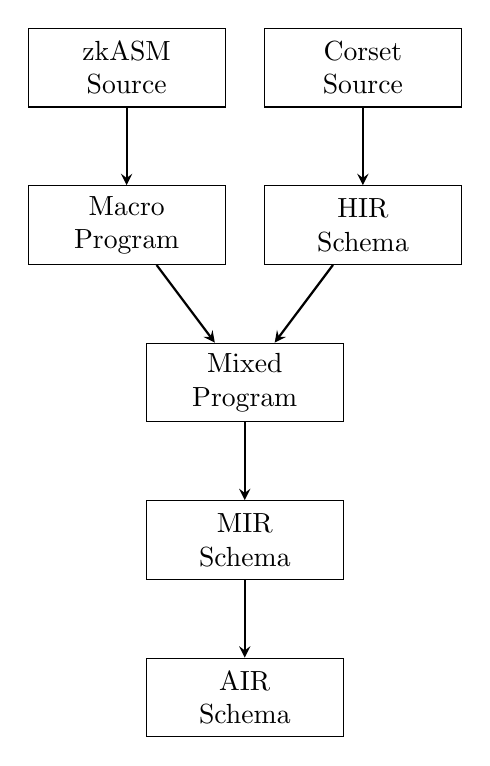
\begin{tikzpicture}[
    node distance=2cm,
    box/.style={rectangle, draw, minimum width=2.5cm, minimum height=1cm, align=center},
    arrow/.style={->, >=stealth, thick}
]
    \node[box] (zkasm) {zkASM\\Source};
    \node[box, right of=zkasm, xshift=1cm] (corset) {Corset\\Source};
    \node[box, below of=zkasm] (macro) {Macro\\Program};
    \node[box, below of=corset] (hir) {HIR\\Schema};
    \node[box, below of=macro, xshift=1.5cm] (mixed) {Mixed\\Program};
    \node[box, below of=mixed] (mir) {MIR\\Schema};
    \node[box, below of=mir] (air) {AIR\\Schema};

    \draw[arrow] (zkasm) -- (macro);
    \draw[arrow] (corset) -- (hir);
    \draw[arrow] (macro) -- (mixed);
    \draw[arrow] (hir) -- (mixed);
    \draw[arrow] (mixed) -- (mir);
    \draw[arrow] (mir) -- (air);
\end{tikzpicture}
\caption{Integration Architecture}
\end{figure}

\subsection{Mixed Program Model}

The \texttt{MixedProgram} combines assembly and external modules:

\begin{lstlisting}[style=golang,caption={MixedProgram Structure}]
type MixedProgram[F, T, M] struct {
    program io.Program[T]  // Assembly functions
    externs []M            // External (Corset) modules
}

func (p *MixedProgram) Modules() Iterator[Module] {
    // Concatenate assembly modules with external modules
    return Chain(p.program.Modules(), p.externs)
}
\end{lstlisting}

\subsection{Module Interface}

Each assembly function implements the schema module interface:

\begin{lstlisting}[style=golang,caption={Module Interface}]
type Module[F] interface {
    Name() string
    Registers() []Register
    Constraints() Iterator[Constraint[F]]
    Assignments() Iterator[Assignment[F]]
}
\end{lstlisting}

\subsection{Constraint Types}

zkASM generates the following constraint types:

\begin{itemize}
    \item \textbf{Vanishing Constraints}: Polynomial equations that must equal zero
    \item \textbf{Range Constraints}: Bit-width proofs for register values
    \item \textbf{Lookup Constraints}: Bus communication verification
\end{itemize}

%==============================================================================
\section{Implementation Details}
%==============================================================================

\subsection{Package Structure}

\begin{verbatim}
pkg/asm/
├── assembler/          # Lexer, parser, linker, validator
│   ├── lexer.go
│   ├── parser.go
│   ├── linker.go
│   └── validation.go
├── compiler/           # Constraint generation
│   ├── compiler.go
│   ├── frame.go       # PC management
│   ├── insn_assign.go # Assignment compilation
│   └── insn_ifgoto.go # Branch compilation
├── io/                 # Core abstractions
│   ├── macro/         # Macro instructions
│   ├── micro/         # Micro instructions
│   ├── executor.go
│   └── state.go
├── program/            # Module wrappers
└── assemble.go         # Pipeline coordinator
\end{verbatim}

\subsection{Key Data Structures}

\subsubsection{Register Representation}

\begin{lstlisting}[style=golang,caption={Register Definition}]
type Register struct {
    Name     string
    Width    uint    // Bit width
    Padding  big.Int // Default/padding value
    IsInput  bool
    IsOutput bool
}

type RegisterId struct {
    Register uint    // Index in function's register list
    Offset   int     // Row offset for shifted access
}
\end{lstlisting}

\subsubsection{Instruction Representation}

\begin{lstlisting}[style=golang,caption={Instruction Structure}]
type Instruction struct {
    Codes []Code  // Sequence of micro codes
}

// Codes execute sequentially until skip=0
type Code interface {
    MicroExecute(state State) (skip uint, pc uint)
}
\end{lstlisting}

\subsection{Branch Table Analysis}

For complex control flow, the compiler builds a branch table:

\begin{lstlisting}[style=golang,caption={Branch Table Construction}]
type BranchTable struct {
    entries []BranchEntry
}

type BranchEntry struct {
    condition Expression  // Guard condition
    target    uint        // Jump target
}

func BuildBranchTable(codes []Code, start uint) BranchTable {
    // Traverse Skip chains to find all reachable targets
    // Build condition for each path
}
\end{lstlisting}

\subsection{Frame Management}

Two framing strategies support different function types:

\textbf{One-Line Framing} (simple functions):
\begin{itemize}
    \item No program counter column needed
    \item All constraints active for every row
    \item Most efficient representation
\end{itemize}

\textbf{Multi-Line Framing} (functions with control flow):
\begin{itemize}
    \item Program counter column tracks execution point
    \item Return flag indicates termination
    \item Constraints guarded by PC value
\end{itemize}

\subsection{Performance Considerations}

\begin{itemize}
    \item \textbf{Vectorization}: Reduces constraint count by merging instructions
    \item \textbf{Instance Caching}: Avoids redundant function executions
    \item \textbf{Lazy Evaluation}: Constraints generated on-demand during compilation
    \item \textbf{Parallel Execution}: Thread-safe instance caching with mutex protection
\end{itemize}

%==============================================================================
\section{Conclusion}
%==============================================================================

zkASM provides a powerful intermediate representation for zero-knowledge circuit programming within the go-corset framework. Key contributions include:

\begin{enumerate}
    \item A clean separation between high-level assembly semantics and low-level constraint generation
    \item Field-agnostic programming through automatic register splitting
    \item Efficient inter-function communication via the bus protocol
    \item Optimization passes including vectorization and unreachable code elimination
\end{enumerate}

The design enables developers to write portable zero-knowledge programs while the compiler handles field-specific adaptations automatically.

%==============================================================================
\appendix
\section{zkASM Grammar}
%==============================================================================

\begin{verbatim}
program     ::= declaration*
declaration ::= constant | include | function

constant    ::= 'const' IDENTIFIER '=' NUMBER
include     ::= 'include' STRING
function    ::= 'fn' IDENTIFIER '(' params ')' '->' '(' returns ')' '{' body '}'

params      ::= param (',' param)*
param       ::= IDENTIFIER ('=' NUMBER)? type
returns     ::= param (',' param)*
type        ::= 'u' NUMBER

body        ::= (label | instruction)*
label       ::= IDENTIFIER ':'
instruction ::= assignment | conditional | jump | return | call

assignment  ::= targets '=' expression
targets     ::= IDENTIFIER (',' IDENTIFIER)*
expression  ::= term (('+' | '-' | '*') term)*
term        ::= NUMBER | IDENTIFIER | '(' expression ')'

conditional ::= 'if' IDENTIFIER cmp_op expression 'goto' IDENTIFIER
cmp_op      ::= '==' | '!=' | '<' | '<=' | '>' | '>='

jump        ::= 'goto' IDENTIFIER
return      ::= 'return'
call        ::= targets '=' IDENTIFIER '(' arguments ')'
arguments   ::= expression (',' expression)*
\end{verbatim}

\end{document}
